\documentclass[aspectratio=169,11pt,table]{beamer}
\usepackage{../assets/ccde-beamer}

%% ---------- Metadatos (plantilla canónica CCDE: \date{} siempre vacío) ----------
\renewcommand{\ccdefootlabel}{CCDE -- Estructura Productiva Regional y Cicatriz COVID-19}
\title{Estructura Productiva Departamental y Vulnerabilidad Macroeconómica en el Perú}
\subtitle{Análisis Composicional (CoDa), Clustering Jerárquico y Efecto Cicatriz Post-COVID-19}
\author{Círculo de Ciencia de Datos y Econometría}
\date{}

\begin{document}

% ================================================================
% PORTADA OFICIAL CCDE (SIN FECHA POR NORMA CANÓNICA)
% ================================================================
\ccdeportada{Estructura Productiva y Cicatriz COVID-19}{Tipología Composicional (CLR/ILR) y Econometría de Panel en los 24 Departamentos del Perú}{CCDE}

% ================================================================
% MAPA DE LA INVESTIGACIÓN Y TESIS CENTRAL (PIRÁMIDE DE MINTO)
% ================================================================
\begin{frame}{Mapa de la Investigación y Tesis Central}
\vspace{-0.08cm}
\begin{columns}[T,onlytextwidth]
\begin{column}{0.53\textwidth}
{\footnotesize\tableofcontents}
\end{column}
\hfill
\begin{column}{0.43\textwidth}
\begin{keybox}[left=2mm,right=2mm,top=1.2mm,bottom=1.2mm,fontupper=\scriptsize\RaggedRight]
\textbf{Tesis Central (Top-Down Takeaway)}\\[0.08cm]
El choque de 2020 paralizó transversalmente todas las regiones ($\approx -14.4\%$), pero la \textbf{hiper-especialización en enclaves mineros} multiplicó por $4.4\times$ la volatilidad histórica y generó una \textbf{cicatriz pospandemia de $-10.92$ puntos} ($p = 0.0029$) entre 2021 y 2023.
\end{keybox}
\vspace{0.10cm}
\begin{ccdebox}[left=2mm,right=2mm,top=1.2mm,bottom=1.2mm]
\scriptsize\RaggedRight
\textbf{Cobertura Empírica}\\
INEI: 24 departamentos, periodo 2008--2025 ($N=428$ obs.\ de panel; 12 sectores productivos).\\[0.06cm]
\textbf{Arsenal Metodológico}\\
CoDa (Aitchison CLR/ILR) + PCA + Ward/K-Means/PAM/GMM + Panel FE con errores clusterizados.
\end{ccdebox}
\end{column}
\end{columns}
\end{frame}

% ================================================================
% SECCIONES MODULARES EMPÍRICAS
% ================================================================
\section{Motivación, Datos e Hipótesis Estructural}

% ================================================================
\begin{frame}{El Dilema Regional ante el Choque COVID-19 (SCQA)}
\vspace{-0.18cm}
\begin{columns}[T,onlytextwidth]
\begin{column}{0.51\textwidth}
\begin{contrastbox}{ccdeblue}{Marco Estructural SCQA}
\scriptsize\RaggedRight
\begin{itemize}\setlength{\itemsep}{0.06em}
  \item \textbf{Situación ($S$):} Los 24 departamentos exhiben fuerte heterogeneidad productiva, desde enclaves mineros ($>40\%$) hasta economías urbanas.
  \item \textbf{Complicación ($C$):} En 2020 el PIB colapsó, pero los modelos en tasas anuales ($\Delta\%\text{PIB}$) sugerían un impacto indiferenciado ($p > 0.20$).
  \item \textbf{Pregunta ($Q$):} ¿Fue el choque neutral a la estructura productiva o las tasas anuales ocultan una cicatriz acumulada asimétrica?
  \item \textbf{Respuesta ($A$):} Al aplicar CoDa (CLR) y pasar a \textbf{niveles indexados ($\text{PIB}_{2019=100}$)}, emerge un rezago pospandemia significativo al $1\%$ en los enclaves.
\end{itemize}
\end{contrastbox}
\end{column}

\begin{column}{0.46\textwidth}
\begin{ccdebox}[left=2mm,right=2mm,top=1mm,bottom=1mm]
\scriptsize
\textbf{\textcolor{ccdenavy}{Arquitectura de la Base Consolidada (INEI)}}
\vspace{0.04cm}

\resizebox{\linewidth}{!}{%
\renewcommand{\arraystretch}{1.10}
\begin{tabular}{@{}l r@{}}
\toprule
\textbf{Dimensión del Panel} & \textbf{Magnitud} \\
\midrule
Unidades transversales ($N$) & \textbf{24 departamentos} \\
Horizonte temporal ($T$) & \textbf{2008--2025 (18 años)} \\
Observaciones totales & \textbf{428 filas de panel} \\
Ventana pre-shock (Clustering) & \textbf{2015--2019 (5 años)} \\
Ventana ciclo COVID (Niveles) & \textbf{2017--2023 (100\% bal.)} \\
Ramas de actividad VAB & \textbf{12 sectores (suma 100\%)} \\
\bottomrule
\end{tabular}%
}
\end{ccdebox}

\vspace{0.05cm}
\begin{keybox}[left=2mm,right=2mm,top=0.9mm,bottom=0.9mm]
\scriptsize\RaggedRight \textbf{So What?}: Clasificar con el promedio 2015--2019 garantiza \textbf{exogeneidad estricta} frente al shock de 2020.
\end{keybox}
\end{column}
\end{columns}
\source{INEI -- Cuentas Nacionales Departamentales (Cuadros 1 y 2, precios constantes de 2007).}
\end{frame}


\section{Geometría Composicional (CoDa) y Tipología Productiva}

% ================================================================
\begin{frame}{Geometría del Simplex: Transformación CLR y PCA}
\vspace{-0.18cm}
\begin{columns}[T,onlytextwidth]
\begin{column}{0.48\textwidth}
\begin{ccdebox}[left=2mm,right=2mm,top=1mm,bottom=1mm]
\scriptsize\RaggedRight
\textbf{1. Cierre Composicional ($\mathcal{S}^D$)}: Las participaciones sectoriales suman $100\%$, induciendo correlaciones negativas espurias en el espacio crudo.\\[0.06cm]
\textbf{2. Reemplazo Multiplicativo}: Lambayeque y San Martín registran $0\%$ en minería (2015--19). Se imputa $\delta = 0.05\%$ reescalando los sectores positivos:
\[
x_{ij}^* = \delta \;\text{(si } x_{ij}=0\text{)}; \quad x_{ij}\!\left(1 - \tfrac{z_i \delta}{100}\right)
\]
\textbf{3. Coordenadas Log-Ratio Centradas (CLR)} con media geométrica $g_i = \big(\prod_{j=1}^D x_{ij}^*\big)^{1/D}$:
\[
\mathrm{clr}(x_i^*) = \left[ \ln\tfrac{x_{i1}^*}{g_i},\, \dots,\, \ln\tfrac{x_{iD}^*}{g_i} \right]
\]
\end{ccdebox}
\end{column}

\begin{column}{0.49\textwidth}
\begin{contrastbox}{ccdemid}{Varianza y Loadings PCA}
\scriptsize
\resizebox{\linewidth}{!}{%
\renewcommand{\arraystretch}{1.08}
\begin{tabular}{@{}l r r r@{}}
\toprule
\textbf{Sector / Métrica} & \textbf{PC1} & \textbf{PC2} & \textbf{PC3} \\
\midrule
\textbf{Varianza Explicada} & \textbf{51.65\%} & \textbf{20.02\%} & \textbf{15.71\%} \\
\textbf{Varianza Acumulada} & \textbf{51.65\%} & \textbf{71.68\%} & \textbf{87.39\%} \\
\midrule
Extracción Minera e Hidroc. & \textcolor{warn}{\textbf{+0.906}} & +0.137 & $-0.241$ \\
Electricidad, Gas y Agua & +0.145 & $-0.289$ & \textcolor{ccdeaccent}{\textbf{+0.825}} \\
Agricultura y Ganadería & $-0.130$ & \textcolor{okgreen}{\textbf{$-0.542$}} & $-0.373$ \\
Manufactura & $-0.152$ & \textcolor{ccdeblue}{\textbf{+0.630}} & +0.212 \\
Comercio & $-0.181$ & +0.016 & $-0.216$ \\
Telecom.\ y Serv.\ Info. & $-0.202$ & +0.217 & $-0.149$ \\
\bottomrule
\end{tabular}%
}
\end{contrastbox}
\vspace{0.05cm}
\begin{keybox}[left=2mm,right=2mm,top=0.9mm,bottom=0.9mm]
\scriptsize\RaggedRight \textbf{Lectura}: \textbf{PC1} mide intensidad extractiva minera (+0.91); \textbf{PC2} opone manufactura (+0.63) contra agro ($-0.54$).
\end{keybox}
\end{column}
\end{columns}
\source{Aitchison (1986); Martín-Fernández et al.\ (2003). Cálculos en \texttt{clustering\_paso1.py}.}
\end{frame}

% ================================================================
\begin{frame}{Validación: CLR+PCA2 Maximiza Silueta y Estabilidad}
\vspace{-0.18cm}
\begin{center}
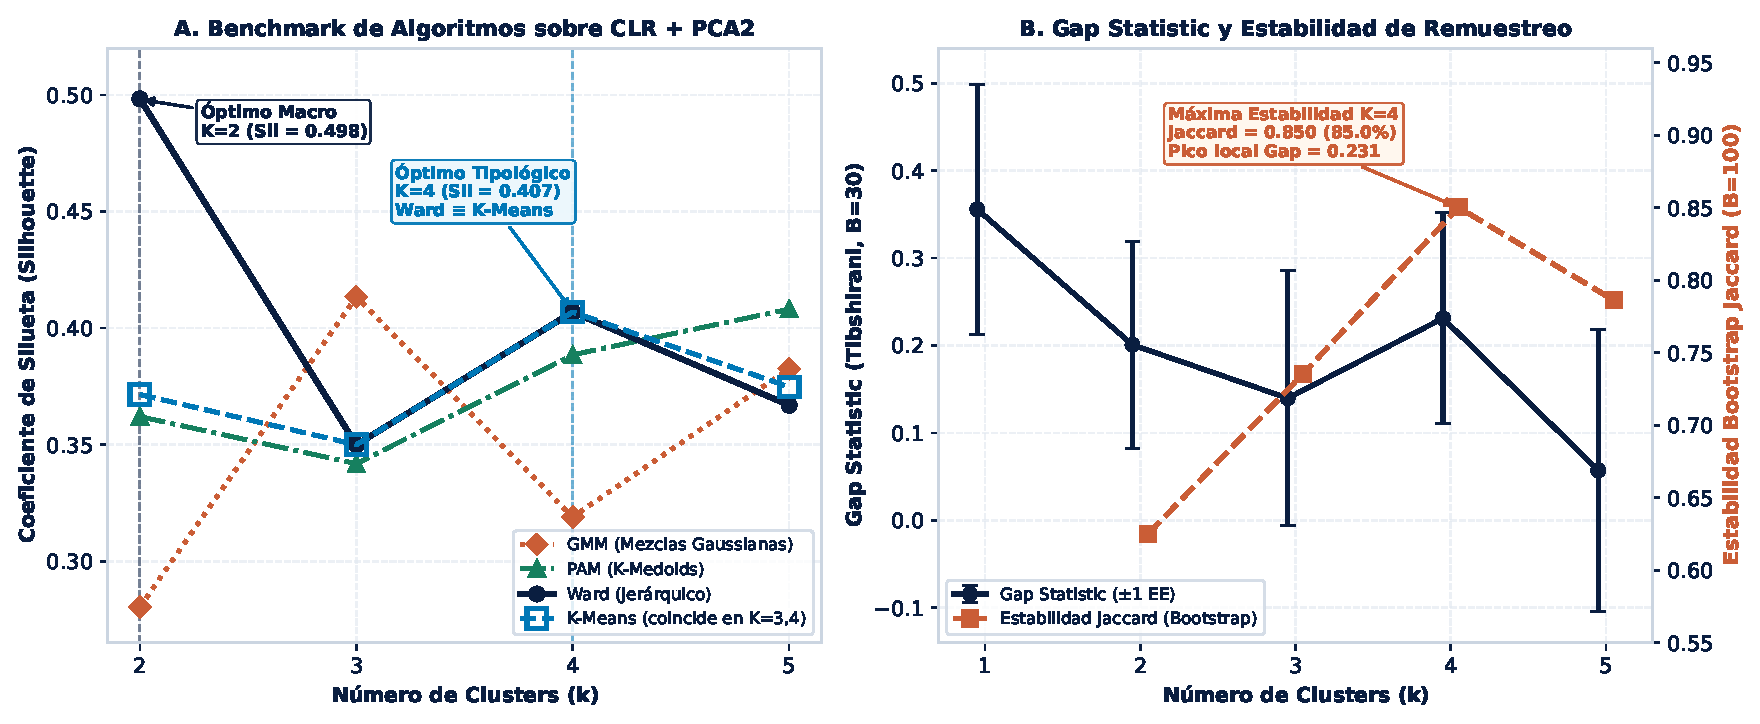
\includegraphics[width=0.88\textwidth,height=0.47\textheight,keepaspectratio]{figures/fig2_validacion_clustering.pdf}
\end{center}
\vspace{-0.24cm}
\begin{columns}[T,onlytextwidth]
\begin{column}{0.59\textwidth}
\begin{ccdebox}[left=2mm,right=2mm,top=0.8mm,bottom=0.8mm]
\scriptsize\RaggedRight
\textbf{Convergencia (48 modelos)}: En $K=4$ sobre CLR+PCA2, \textbf{Ward} y \textbf{K-Means} producen la misma partición ($\text{Silueta}=0.407$, $\text{CH}=22.24$), superando a PAM ($0.389$) y GMM ($0.319$).
\end{ccdebox}
\end{column}
\begin{column}{0.38\textwidth}
\begin{keybox}[left=2mm,right=2mm,top=0.8mm,bottom=0.8mm]
\scriptsize\RaggedRight \textbf{Doble Óptimo}: $K=2$ lidera en silueta ($0.498$) y $K=4$ maximiza estabilidad Jaccard ($85.0\%\text{--}87.7\%$).
\end{keybox}
\end{column}
\end{columns}
\source{Tibshirani et al.\ (2001) para Gap Statistic ($B=30$); Hennig (2007) para estabilidad Jaccard ($B=100$).}
\end{frame}

% ================================================================
\begin{frame}{Mapa Estructural: Cuatro Perfiles en CLR + PCA}
\vspace{-0.14cm}
\begin{columns}[c,onlytextwidth]
\begin{column}{0.65\textwidth}
\centering
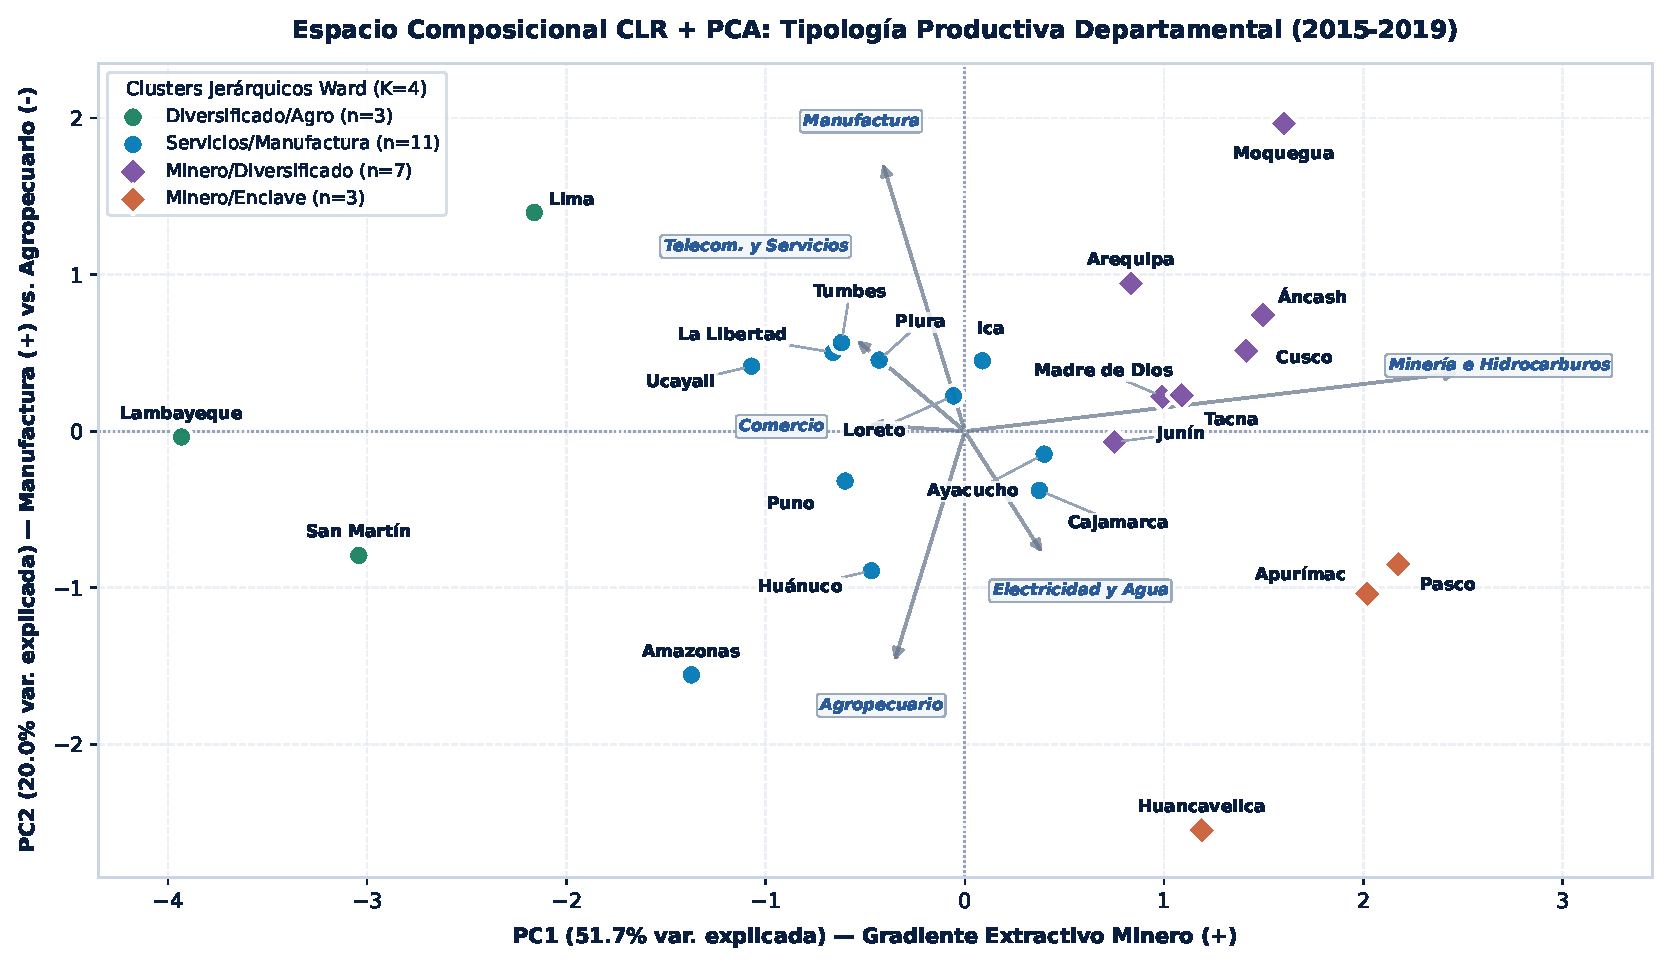
\includegraphics[width=\linewidth,height=0.66\textheight,keepaspectratio]{figures/fig1_pca_biplot_clusters.pdf}
\end{column}
\begin{column}{0.33\textwidth}
\begin{ccdebox}[left=2mm,right=2mm,top=1mm,bottom=1mm]
\scriptsize\RaggedRight
\textbf{\textcolor{ccdenavy}{Geometría de los 4 Clusters}}\\[0.05cm]
\textcolor{warn}{$\blacklozenge$ \textbf{Minero/Enclave ($n=3$):}}\\
Apurímac, Pasco y Huancavelica (alta extracción + energía).\\[0.05cm]
\textcolor{purplex}{$\blacklozenge$ \textbf{Minero/Diversificado ($n=7$):}}\\
Moquegua, Áncash, Cusco, Arequipa, Tacna, Madre de Dios y Junín.\\[0.05cm]
\textcolor{ccdeaccent}{$\bullet$ \textbf{Servicios/Manufactura ($n=11$):}}\\
Núcleo central (Ica, La Libertad, Piura, Cajamarca, Puno, etc.).\\[0.05cm]
\textcolor{okgreen}{$\bullet$ \textbf{Diversificado/Agro ($n=3$):}}\\
Lima, Lambayeque y San Martín en el extremo no minero ($PC1 < -2$).
\end{ccdebox}
\end{column}
\end{columns}
\source{Elaboración propia sobre el promedio composicional 2015--2019 (\texttt{modelo-clusters.ipynb}).}
\end{frame}

% ================================================================
\begin{frame}{Anatomía Jerárquica: $K=4$ Anidado dentro de $K=2$}
\vspace{-0.18cm}
\begin{center}
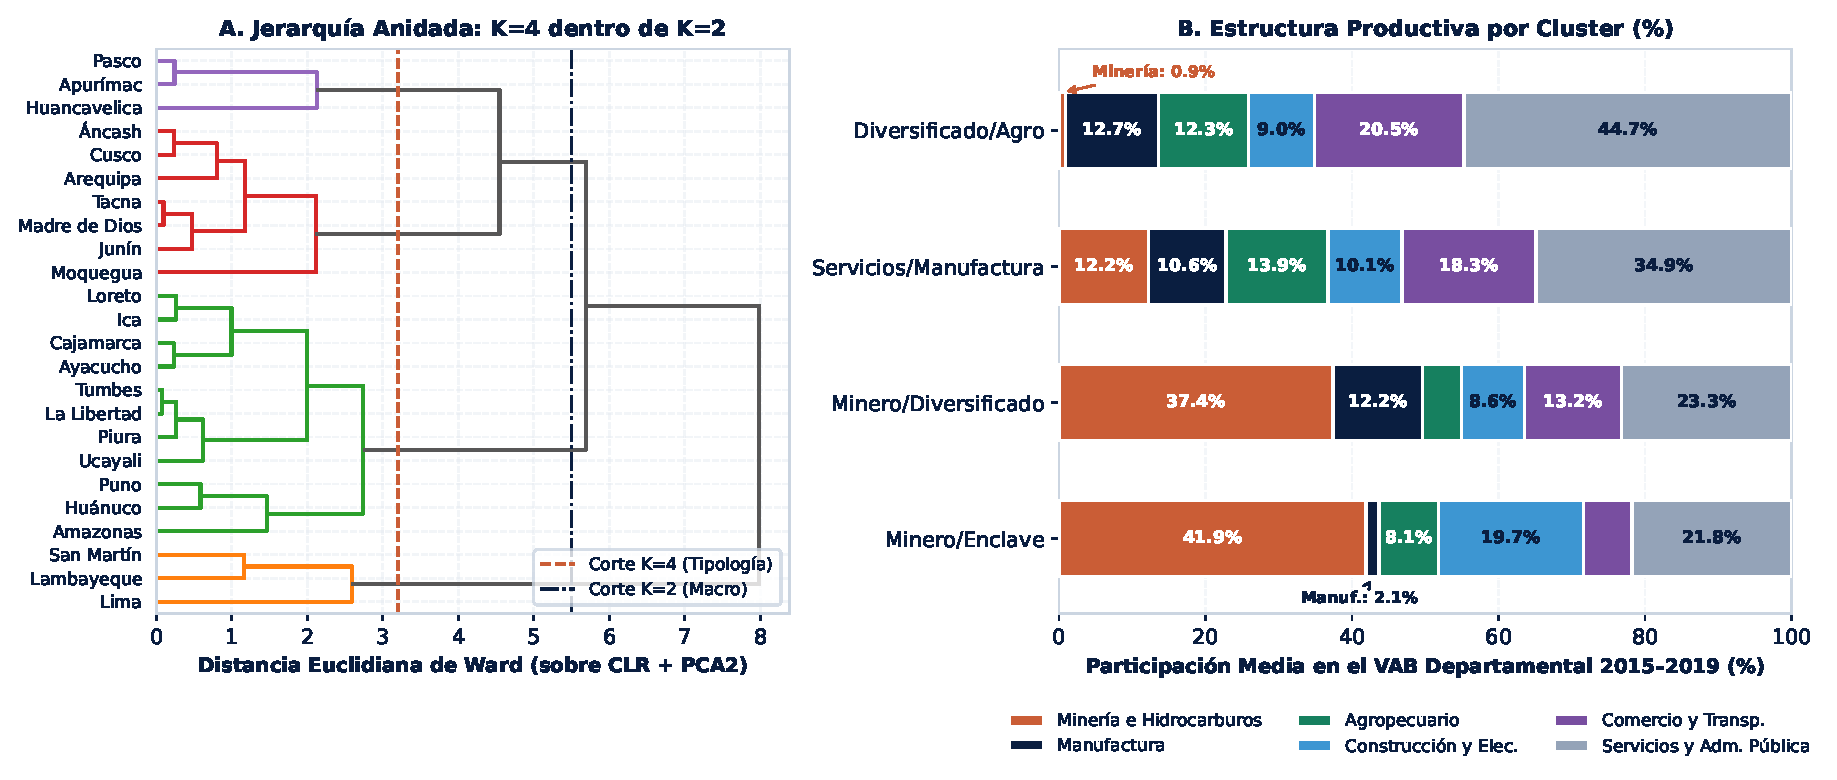
\includegraphics[width=0.90\textwidth,height=0.50\textheight,keepaspectratio]{figures/fig3_dendrograma_perfiles.pdf}
\end{center}
\vspace{-0.24cm}
\begin{keybox}[left=2mm,right=2mm,top=0.8mm,bottom=0.8mm]
\scriptsize\RaggedRight
\textbf{Anidamiento exacto de Ward}: Los 4 clusters se agrupan sin cruces en dos bloques macroeconómicos: \textbf{Bloque Minero} ($N=10$: \textit{Enclave} $41.9\%$ minería + \textit{Minero/Div.} $37.4\%$ minería) vs.\ \textbf{Bloque Diversificado} ($N=14$: \textit{Serv./Manuf.} $12.2\%$ + \textit{Div./Agro} $0.9\%$).
\end{keybox}
\source{Resultados en \texttt{clustering\_paso4\_perfil\_K4.xlsx} y \texttt{econ\_reagrupa.py}.}
\end{frame}

\section{Régimen de Volatilidad Estructural e Ilusión del Efecto Base}

% ================================================================
\begin{frame}{Riesgo Regional: Enclaves Exhiben $4.4\times$ Más Volatilidad}
\vspace{-0.18cm}
\begin{center}
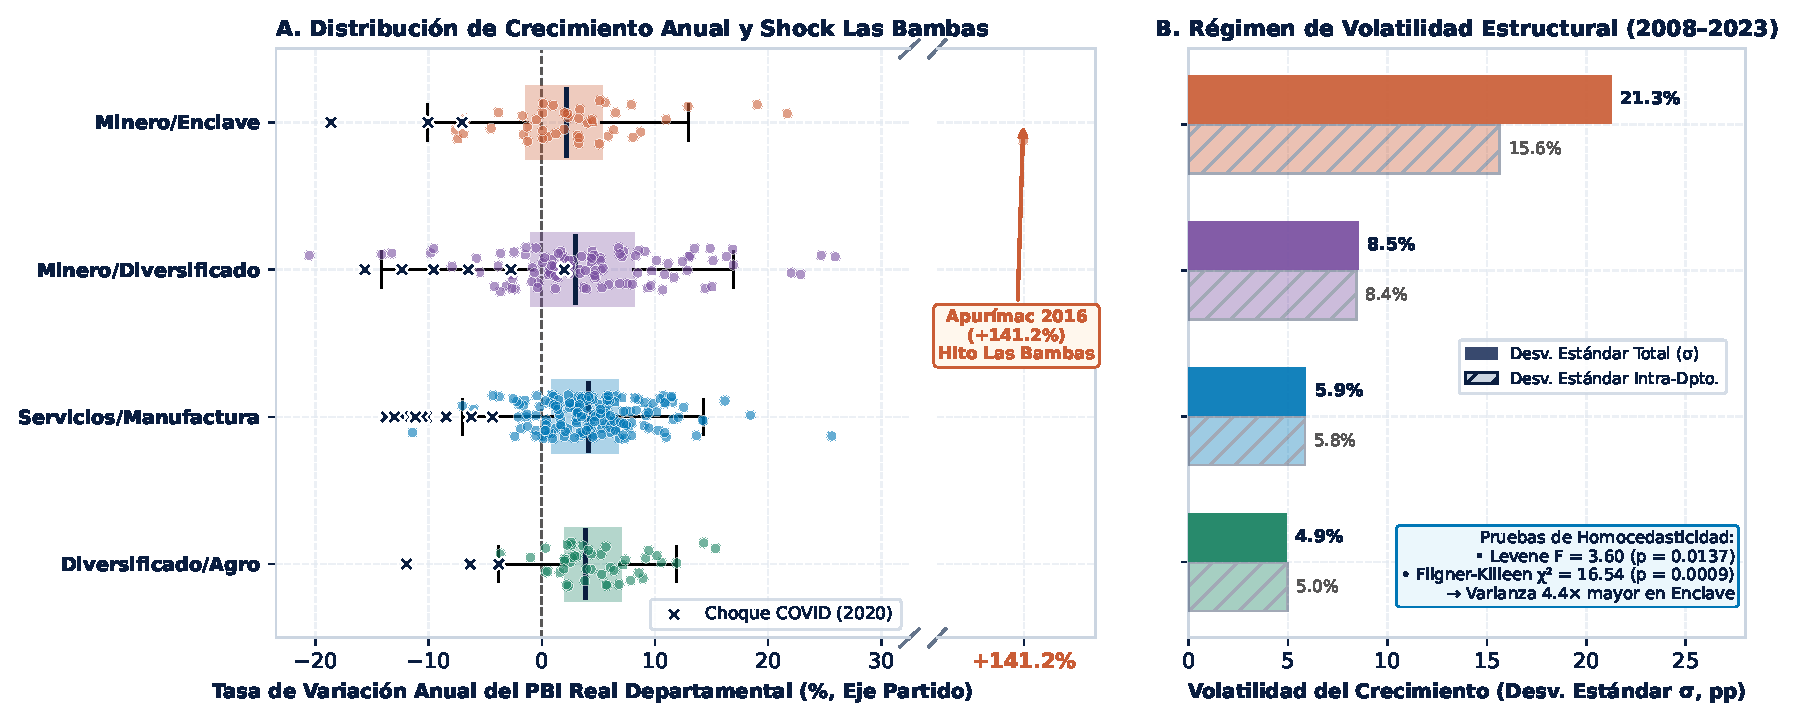
\includegraphics[width=0.89\textwidth,height=0.47\textheight,keepaspectratio]{figures/fig4_volatilidad_estructural.pdf}
\end{center}
\vspace{-0.24cm}
\begin{columns}[T,onlytextwidth]
\begin{column}{0.56\textwidth}
\begin{ccdebox}[left=2mm,right=2mm,top=0.8mm,bottom=0.8mm]
\scriptsize\RaggedRight
\textbf{Heterocedasticidad verificada}: El test de \textbf{Levene} ($F=3.97, p=0.0083$) y \textbf{Fligner-Killeen} ($\chi^2=17.54, p=0.0005$) confirman varianzas dispares ($\sigma = 20.5\%$ en Enclave vs.\ $4.6\%$ en Agro).
\end{ccdebox}
\end{column}
\begin{column}{0.41\textwidth}
\begin{keybox}[left=2mm,right=2mm,top=0.8mm,bottom=0.8mm]
\scriptsize\RaggedRight \textbf{Shock Las Bambas (2016)}: Apurímac creció $+141.2\%$ en un año, inflando la varianza residual en tasas.
\end{keybox}
\end{column}
\end{columns}
\source{Panel 2008--2025 ($N=428$). Pruebas de varianza ejecutadas en \texttt{modelo-econometrico.ipynb}.}
\end{frame}

% ================================================================
\begin{frame}{El Puzzle de las Tasas Anuales (Modelos M1--M4)}
\vspace{-0.14cm}
\begin{columns}[T,onlytextwidth]
\begin{column}{0.56\textwidth}
\begin{ccdebox}[left=2mm,right=2mm,top=1.1mm,bottom=1.1mm]
\scriptsize
\textbf{\textcolor{ccdenavy}{Panel FE sobre Crecimiento Anual ($\text{var\_pib}_{it}$, 2008--2025)}}
\vspace{0.04cm}

\resizebox{\linewidth}{!}{%
\renewcommand{\arraystretch}{1.10}
\begin{tabular}{@{}l r r r r@{}}
\toprule
\textbf{Variable / Estadístico} & \textbf{M1 ($K=4$)} & \textbf{M2 (Macro)} & \textbf{M3 (+Rebote)} & \textbf{M4 (Sin Apu16)} \\
\midrule
Intercepto ($\hat{\alpha}$) & $4.53^{***}$ & $4.53^{***}$ & $4.12^{***}$ & $4.19^{***}$ \\
$\text{COVID}_{2020}$ (Base) & $-11.95^{***}$ & $-14.43^{***}$ & $-13.97^{***}$ & $-14.43^{***}$ \\
$\text{REBOTE}_{2021}$ (Base) & --- & --- & $+7.80^{***}$ & --- \\
\midrule
$\text{COVID} \times \text{Serv./Manuf.}$ & $-2.90$ (0.20) & --- & --- & --- \\
$\text{COVID} \times \text{Minero/Div.}$ & $-1.70$ (0.64) & --- & --- & --- \\
$\text{COVID} \times \text{Minero/Enclave}$ & $-5.73$ (0.13) & --- & --- & --- \\
$\text{COVID} \times \text{Macro Minero}$ & --- & $-0.63$ (0.81) & $-0.75$ (0.77) & $+0.28$ (0.91) \\
$\text{REBOTE} \times \text{Macro Minero}$ & --- & --- & $-2.11$ (0.45) & --- \\
\midrule
Observaciones ($N$) & 428 & 428 & 428 & 427 \\
$R^2$ Within & 0.1390 & 0.1376 & 0.1691 & \textcolor{okgreen}{\textbf{0.2620}} \\
Poolability $F$ ($p$-valor) & 0.96 (0.51) & 0.92 (0.57) & 0.96 (0.52) & 1.07 (0.38) \\
\bottomrule
\end{tabular}%
}
\vspace{0.02cm}
{\tiny Nota: $p$-valores con errores estándar clusterizados entre paréntesis. $^{***}p<0.01$.}
\end{ccdebox}
\end{column}

\begin{column}{0.41\textwidth}
\begin{contrastbox}{warn}{Diagnóstico del Puzzle}
\scriptsize\RaggedRight
\begin{enumerate}\setlength{\itemsep}{0.10em}
  \item \textbf{Parálisis transversal (Q2-2020):} El confinamiento detuvo tanto la gran minería como el comercio ($\approx -14.4\%$).
  \item \textbf{Ruido pre-pandemia:} En M4, excluir solo \textit{Apurímac 2016} casi duplica el $R^2_{\text{within}}$ ($13.8\% \rightarrow 26.2\%$).
  \item \textbf{Ilusión del efecto base:} Caer $-12\%$ en 2020 y crecer $+9\%$ en 2021 luce positivo en $\text{var\_pib}$, pero deja al PIB en $95.9\%$ del nivel de 2019.
\end{enumerate}
\end{contrastbox}
\vspace{0.04cm}
\begin{keybox}[left=2mm,right=2mm,top=0.8mm,bottom=0.8mm]
\scriptsize\RaggedRight \textbf{Solución}: Modelar el \textbf{nivel acumulado indexado ($\text{PIB}_{2019=100}$)}.
\end{keybox}
\end{column}
\end{columns}
\source{Estimaciones con \texttt{linearmodels.PanelOLS} en \texttt{econ\_paso1.py} a \texttt{econ\_paso3.py}.}
\end{frame}


\section{Evidencia en Niveles Indexados y Efecto Cicatriz (Scarring Effect)}

% ================================================================
\begin{frame}{Trayectoria Indexada ($\text{PIB}_{2019=100}$): Cicatriz en Enclaves}
\vspace{-0.18cm}
\begin{center}
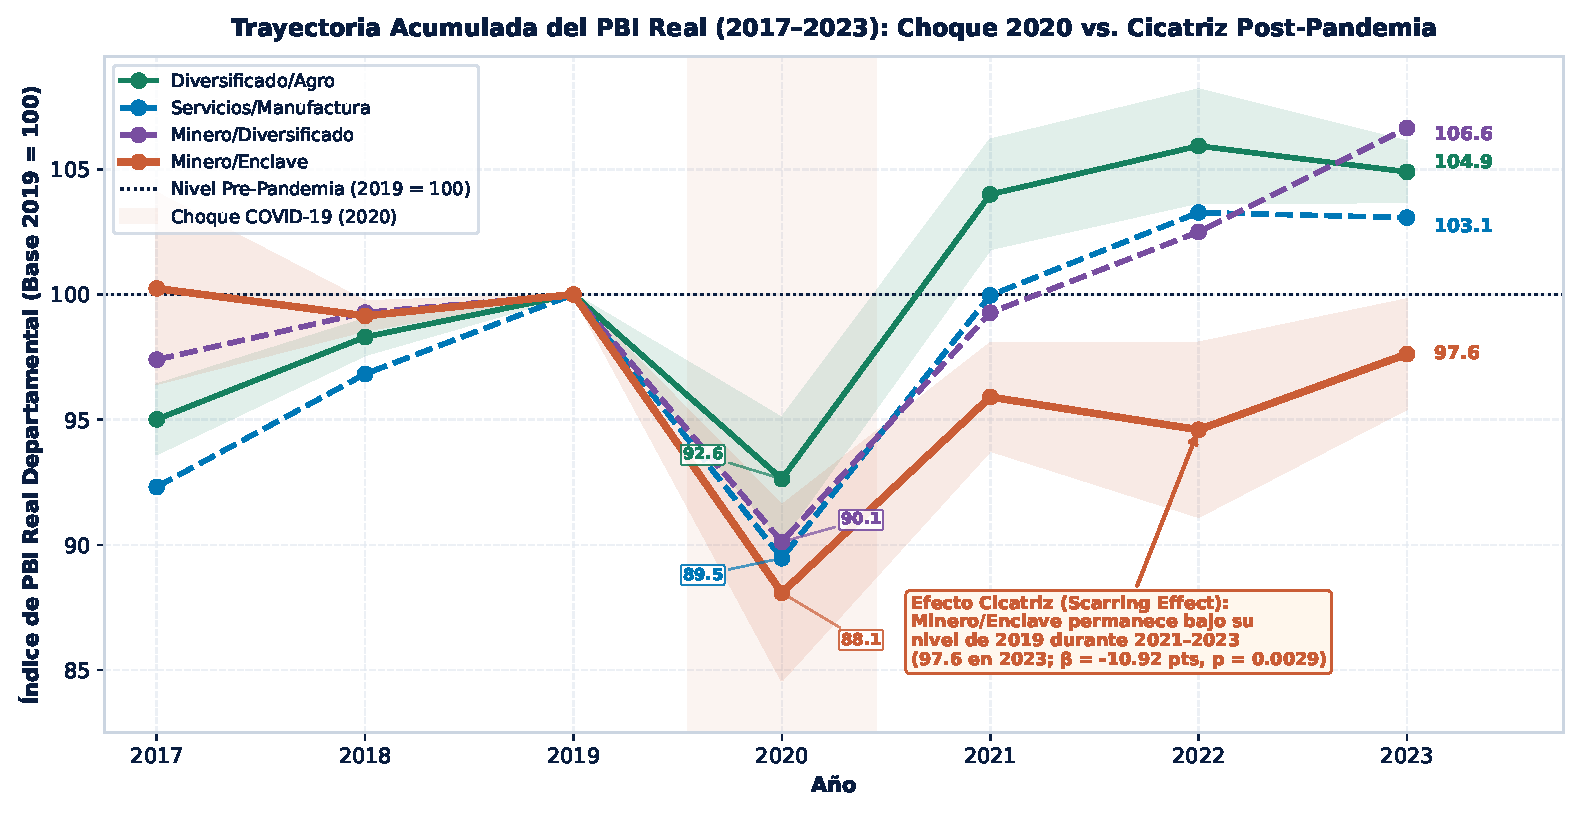
\includegraphics[width=0.86\textwidth,height=0.47\textheight,keepaspectratio]{figures/fig5_trayectoria_pib_indexado.pdf}
\end{center}
\vspace{-0.24cm}
\begin{columns}[T,onlytextwidth]
\begin{column}{0.58\textwidth}
\begin{ccdebox}[left=2mm,right=2mm,top=0.8mm,bottom=0.8mm]
\scriptsize\RaggedRight
\textbf{Divergencia 2021--2023}: \textit{Diversificado/Agro} ($104.9$), \textit{Minero/Div.} ($106.6$) y \textit{Serv./Manuf.} ($103.1$) superaron el nivel de 2019; \textbf{Minero/Enclave quedó bajo 100 todo el trienio ($95.9 \rightarrow 94.6 \rightarrow 97.6$)}.
\end{ccdebox}
\end{column}
\begin{column}{0.39\textwidth}
\begin{keybox}[left=2mm,right=2mm,top=0.8mm,bottom=0.8mm]
\scriptsize\RaggedRight \textbf{Mecanismo}: Conflictividad en el Corredor Minero y baja articulación local frenaron la recuperación.
\end{keybox}
\end{column}
\end{columns}
\source{Panel balanceado 2017--2023 ($N=24, T=7, \text{Obs}=168$). Elaboración propia (\texttt{generar\_analisis\_completo.py}).}
\end{frame}

% ================================================================
\begin{frame}{Modelos en Nivel Indexado (M5--M6): Cicatriz al 1\%}
\vspace{-0.14cm}
\begin{columns}[T,onlytextwidth]
\begin{column}{0.57\textwidth}
\begin{ccdebox}[left=2mm,right=2mm,top=1mm,bottom=1mm]
\scriptsize
\textbf{\textcolor{ccdenavy}{Dependiente: Índice de PIB Real ($\text{PIB}_{i,2019}=100$, 2017--2023)}}
\vspace{0.03cm}

\resizebox{\linewidth}{!}{%
\renewcommand{\arraystretch}{1.06}
\begin{tabular}{@{}l r r r r@{}}
\toprule
& \multicolumn{2}{c}{\textbf{M5: Clusters ($K=4$)}} & \multicolumn{2}{c}{\textbf{M6: Continuo ($\text{Minería}_z$)}} \\
\cmidrule(lr){2-3}\cmidrule(lr){4-5}
\textbf{Regresor (Efectos Fijos)} & \textbf{Beta} & \textbf{$p$-valor} & \textbf{Beta} & \textbf{$p$-valor} \\
\midrule
Intercepto (Senda Pre-COVID) & $97.71^{***}$ & 0.0000 & $97.71^{***}$ & 0.0000 \\
$\text{COVID}_{2020}$ (Ref: Div./Agro) & $-5.14^{***}$ & 0.0016 & $-7.83^{***}$ & 0.0000 \\
$\text{POST}_{2021\text{--}23}$ (Ref: Div./Agro) & $+7.17^{***}$ & 0.0000 & $+4.19^{**}$ & 0.0224 \\
\midrule
$\text{COVID}_{2020} \times \text{Serv./Manuf.}$ & $-1.77$ & 0.3318 & --- & --- \\
$\text{COVID}_{2020} \times \text{Minero/Div.}$ & $-3.63$ & 0.4655 & --- & --- \\
\rowcolor{warn!12}
$\text{COVID}_{2020} \times \text{Minero/Enclave}$ & \textcolor{warn}{$\mathbf{-6.57^{**}}$} & \textcolor{warn}{\textbf{0.0495}} & --- & --- \\
$\text{POST}_{2021\text{--}23} \times \text{Serv./Manuf.}$ & $-1.45$ & 0.5212 & --- & --- \\
$\text{POST}_{2021\text{--}23} \times \text{Minero/Div.}$ & $-3.26$ & 0.5694 & --- & --- \\
\rowcolor{warn!18}
$\text{POST}_{2021\text{--}23} \times \text{Minero/Enclave}$ & \textcolor{warn}{$\mathbf{-10.92^{***}}$} & \textcolor{warn}{\textbf{0.0029}} & --- & --- \\
\rowcolor{ccdelight!22}
$\text{COVID}_{2020} \times \text{Minería}_z$ (1 SD) & --- & --- & \textcolor{ccdeblue}{$\mathbf{-2.39^{*}}$} & \textcolor{ccdeblue}{\textbf{0.0891}} \\
\rowcolor{ccdelight!22}
$\text{POST}_{2021\text{--}23} \times \text{Minería}_z$ (1 SD) & --- & --- & \textcolor{ccdeblue}{$\mathbf{-2.76^{*}}$} & \textcolor{ccdeblue}{\textbf{0.0747}} \\
\midrule
Observaciones / Departamentos & \multicolumn{2}{c}{168 / 24} & \multicolumn{2}{c}{168 / 24} \\
$R^2$ Within & \multicolumn{2}{c}{\textcolor{okgreen}{\textbf{0.3554}}} & \multicolumn{2}{c}{\textcolor{okgreen}{\textbf{0.3451}}} \\
Test $F$ Poolability ($p$-valor) & \multicolumn{2}{c}{\textbf{3.14 ($p < 0.0001$)}} & \multicolumn{2}{c}{\textbf{3.29 ($p < 0.0001$)}} \\
\bottomrule
\end{tabular}%
}
\end{ccdebox}
\end{column}

\begin{column}{0.40\textwidth}
\begin{contrastbox}{okgreen}{Salto Econométrico}
\scriptsize\RaggedRight
\begin{itemize}\setlength{\itemsep}{0.12em}
  \item \textbf{Efectos fijos validados:} El test de Poolability pasa de $p=0.51$ (en tasas) a \textbf{$p < 0.0001$} en niveles indexados.
  \item \textbf{Mayor ajuste:} El $R^2_{\text{within}}$ sube de $13.9\%$ a \textbf{$35.5\%$}.
  \item \textbf{Doble golpe al Enclave (M5):} Caída adicional de \textbf{$-6.57$ pts} en 2020 ($p=0.0495$) y rezago acumulado de \textbf{$-10.92$ pts} en 2021--2023 ($p=0.0029$).
  \item \textbf{Gradiente continuo (M6):} $+1\text{ SD}$ en minería reduce el nivel pospandemia en \textbf{$-2.76$ pts} ($p=0.075$).
\end{itemize}
\end{contrastbox}
\end{column}
\end{columns}
\source{Estimaciones PanelOLS con efectos fijos de entidad y errores estándar clusterizados (\texttt{resumen\_modelos\_econometricos.xlsx}).}
\end{frame}

% ================================================================
\begin{frame}{Contraste de Modelos: Tasas Anuales vs. Niveles}
\vspace{-0.18cm}
\begin{center}
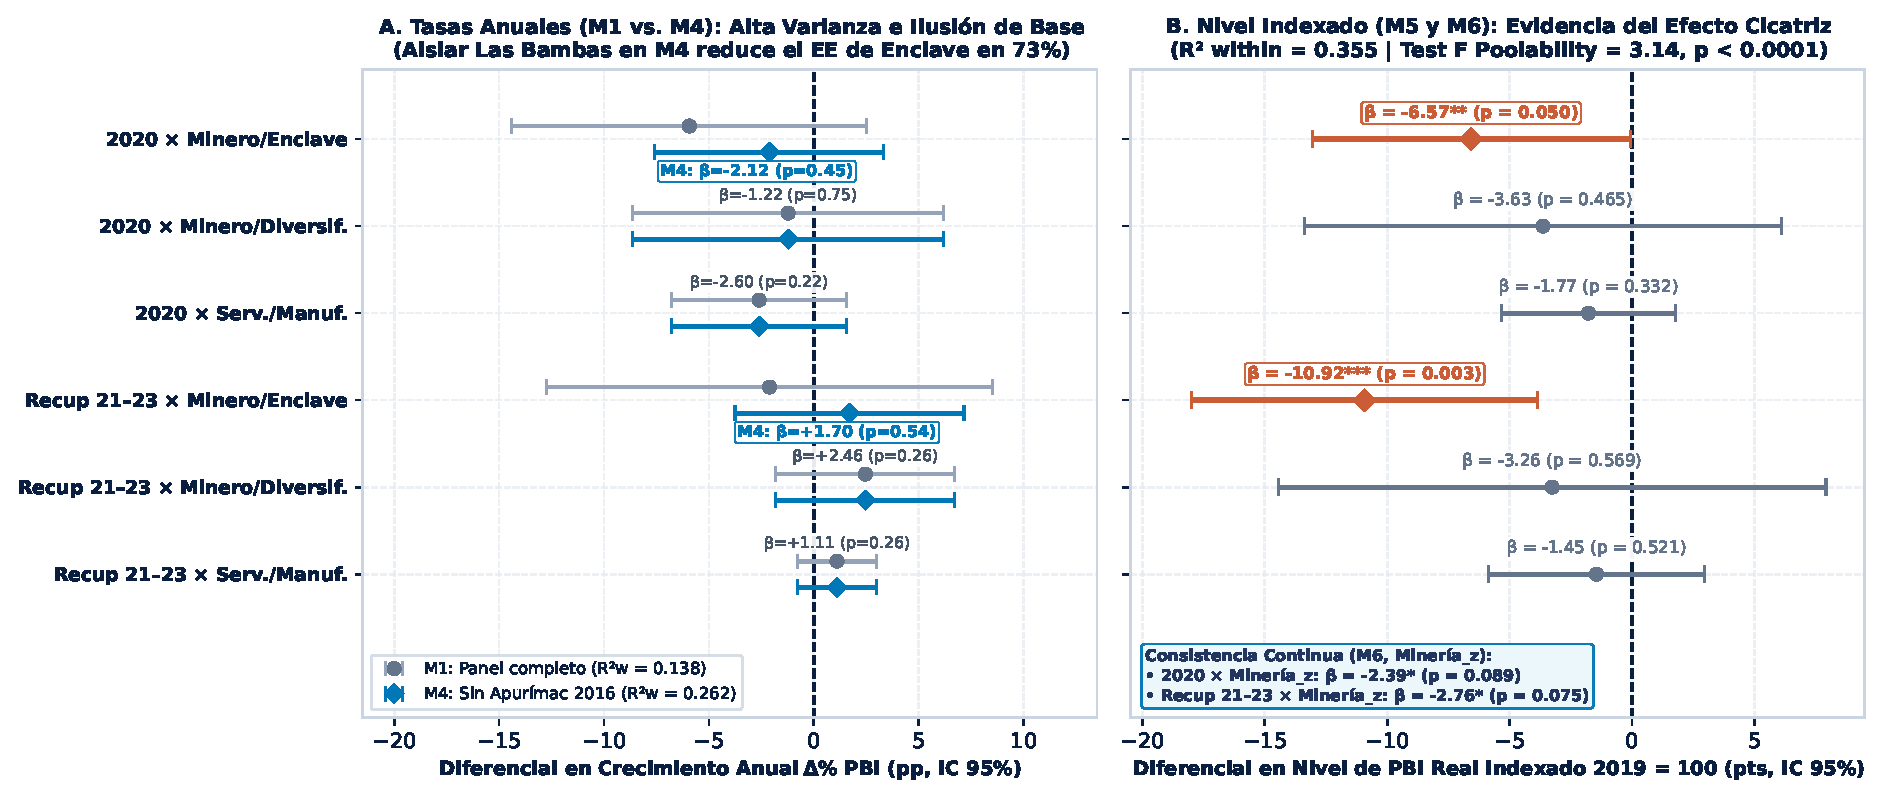
\includegraphics[width=0.90\textwidth,height=0.50\textheight,keepaspectratio]{figures/fig6_forest_plot_modelos.pdf}
\end{center}
\vspace{-0.24cm}
\begin{keybox}[left=2mm,right=2mm,top=0.8mm,bottom=0.8mm]
\scriptsize\RaggedRight
\textbf{Lección metodológica}: Evaluar choques estructurales mediante variaciones interanuales aisladas (Panel A) induce un \textbf{error Tipo II} (falso negativo). La especificación en nivel acumulado $\text{PIB}_{2019=100}$ (Panel B) revela la persistencia real del daño productivo.
\end{keybox}
\source{Intervalos de confianza al 95\% basados en errores estándar robustos agrupados por departamento.}
\end{frame}


\section{Conclusiones, Implicancias y Reproducibilidad}

% ================================================================
\begin{frame}{Conclusiones e Implicancias de Política Regional}
\vspace{-0.18cm}
\begin{columns}[T,onlytextwidth]
\begin{column}{0.48\textwidth}
\begin{contrastbox}{ccdenavy}{Hallazgos Empíricos Centrales}
\scriptsize\RaggedRight
\begin{enumerate}\setlength{\itemsep}{0.06em}
  \item \textbf{Jerarquía dual ($K=4 \subset K=2$):} CLR+PCA2 divide al país en un bloque Minero ($N=10$) y uno Diversificado ($N=14$), subdivididos con $85\%$ de estabilidad bootstrap en 4 perfiles.
  \item \textbf{Minería Diversificada vs.\ Enclave:} \textit{Minero/Div.} (Arequipa, Moquegua, Cusco) superó su nivel pre-COVID ($106.6$ en 2023), pero \textit{Minero/Enclave} (Apurímac, Pasco, Huancavelica) sufrió una cicatriz de $-10.92$ pts ($p=0.0029$).
  \item \textbf{Trampa de volatilidad:} Los enclaves soportan una volatilidad ($\sigma=20.5\%$) $4.4\times$ mayor que el grupo agro/servicios ($\sigma=4.6\%$).
\end{enumerate}
\end{contrastbox}
\end{column}

\begin{column}{0.48\textwidth}
\begin{contrastbox}{okgreen}{Agenda de Política Regional}
\scriptsize\RaggedRight
\begin{itemize}\setlength{\itemsep}{0.04em}
  \item \textbf{Encadenamientos en enclaves:} Invertir canon en Apurímac, Pasco y Huancavelica en agroindustria y logística que amortigüen paros extractivos.
  \item \textbf{Fondos de estabilización:} Reglas contracíclicas en clusters con $\sigma > 15\%$ para suavizar inversión pública.
  \item \textbf{Métrica en niveles:} Evaluar desempeño con índices acumulados ($\text{PIB}_{2019=100}$) en vez de tasas anuales.
\end{itemize}
\end{contrastbox}
\vspace{0.03cm}
\begin{keybox}[left=2mm,right=2mm,top=0.6mm,bottom=0.6mm]
\scriptsize\RaggedRight \textbf{Mensaje Final}: La fragilidad pospandemia proviene de la \textbf{falta de diversificación} en economías de enclave.
\end{keybox}
\end{column}
\end{columns}
\source{Síntesis del equipo de investigación -- Círculo de Ciencia de Datos y Econometría (CCDE).}
\end{frame}

% ================================================================
\begin{frame}{Trazabilidad Reproducible y Referencias Clave}
\vspace{-0.14cm}
\begin{columns}[T,onlytextwidth]
\begin{column}{0.51\textwidth}
\begin{ccdebox}[left=2mm,right=2mm,top=1mm,bottom=1mm]
\scriptsize
\textbf{\textcolor{ccdenavy}{Arquitectura del Repositorio}}
\vspace{0.04cm}

\resizebox{\linewidth}{!}{%
\renewcommand{\arraystretch}{1.10}
\begin{tabular}{@{}l l@{}}
\toprule
\textbf{Módulo / Archivo} & \textbf{Función en el Pipeline} \\
\midrule
\texttt{src/generador-df.py} & ETL de 24 Excels INEI $\rightarrow$ panel base \\
\texttt{src/clustering\_paso1..4.py} & Ceros $\delta=0.05$, CLR/ILR, PCA y Gap \\
\texttt{src/econ\_paso1..3.py} & Modelos en tasas y diagnóstico $K=2$ \\
\texttt{src/generar\_analisis\_completo.py} & Modelos M1--M6 en niveles y 6 figuras \\
\texttt{src/modelo-clusters.ipynb} & Cuaderno ejecutable de tipología CoDa \\
\texttt{src/modelo-econometrico.ipynb} & Cuaderno ejecutable de Panel FE \\
\texttt{data/processed/*.xlsx} & Bases (\texttt{panel\_econometrico\_final}) \\
\bottomrule
\end{tabular}%
}
\end{ccdebox}
\vspace{0.05cm}
\begin{keybox}[left=2mm,right=2mm,top=0.9mm,bottom=0.9mm]
\scriptsize\RaggedRight \textbf{Reproducibilidad}: Semilla fija (\texttt{RANDOM\_STATE = 0}), entorno declarativo en \texttt{requirements.txt} y trazabilidad en Git.
\end{keybox}
\end{column}

\begin{column}{0.46\textwidth}
\begin{ccdebox}[left=2mm,right=2mm,top=1mm,bottom=1mm]
\scriptsize\RaggedRight
\textbf{\textcolor{ccdenavy}{Referencias Metodológicas Clave}}
\vspace{0.05cm}

\textbf{Aitchison, J.} \textcolor{ccdemid}{(1986)}. \textit{The Statistical Analysis of Compositional Data}. Chapman \& Hall.\\[0.06cm]
\textbf{Martín-Fernández, J. A. et al.} \textcolor{ccdemid}{(2003)}. Dealing with zeros in compositional data sets. \textit{Math.\ Geol.}, 35(3), 253--278.\\[0.06cm]
\textbf{Tibshirani, R., Walther, G. \& Hastie, T.} \textcolor{ccdemid}{(2001)}. Estimating the number of clusters via the gap statistic. \textit{JRSS-B}, 63(2), 411--423.\\[0.06cm]
\textbf{Wooldridge, J. M.} \textcolor{ccdemid}{(2010)}. \textit{Econometric Analysis of Cross Section and Panel Data}. MIT Press.\\[0.06cm]
\textbf{INEI} \textcolor{ccdemid}{(2025)}. \textit{Producto Bruto Interno por Departamentos 2007--2025}. Lima.
\end{ccdebox}
\end{column}
\end{columns}
\source{Repositorio oficial: \texttt{https://github.com/CCDE-DataLab/clusters-departamentales}.}
\end{frame}

\end{document}

